% % % % % % % % % % % % % % % % % % % % % % % % % % % % % % % % % % % % % % % % % % % %
%                                                                                     %
% Short Sectioned Assignment LaTeX Template Version 1.0 (5/5/12)                      %
% This template has been downloaded from: http://www.LaTeXTemplates.com               %
%                                                                                     %
% Original author:  Frits Wenneker (http://www.howtotex.com)                          %
%                                                                                     %
% Modified by: Fco Javier Sueza Rodríguez (fcosueza@disroot.org)                      %
%                                                                                     %
% Changes:                                                                            %
%	    - Custom Chapters, Sections and Subsections (titlesec package)                %
%           - Document type scrbook (oneside)                                         %
%           - Use babel-lang-spanish package and marvosym                             %
%           - Use hyperref, enumitem, tcolorbox and glossaries packages               %
%           - Use Time New Roman (mathptmx), Helvetic and Courier fonts               %
%                                                                                     %
% License: CC BY-NC-SA 3.0 (http://creativecommons.org/licenses/by-nc-sa/3.0/)        %
%                                                                                     %
% % % % % % % % % % % % % % % % % % % % % % % % % % % % % % % % % % % % % % % % % % % %

%-----------------------------------------------%
%	              Packages                  %
%-----------------------------------------------%

\documentclass[paper=a4, fontsize=11pt, oneside]{scrbook}

% ---- Text Input/Output ----- %

\usepackage[T1]{fontenc}
\usepackage[utf8]{inputenc}
\usepackage{mathptmx}
\usepackage[scaled=.92]{helvet}
\usepackage{courier}
\usepackage[indent=12pt]{parskip}

\usepackage{geometry}
\geometry{verbose,tmargin=3cm,bmargin=3cm,lmargin=2.6cm,rmargin=2.6cm}

% ---- Language ----- %

\usepackage[spanish]{babel}
\usepackage{marvosym}

% ---- Another packages ---- %

\usepackage{amsmath,amsfonts,amsthm}
\usepackage{graphics,graphicx}
\usepackage{titlesec}
\usepackage{fancyhdr}
\usepackage{tcolorbox}
\usepackage{hyperref}
\usepackage{enumitem}
\usepackage[automake]{glossaries}

%--------------------------------------------------------------------%
%                      Customizing Document                          %
%--------------------------------------------------------------------%


% ----------- Custom Chapters, Sections and Subsections -------------- %

\titleformat{\chapter}[display]
			{\bfseries\Huge}
			{Tema \ \thechapter} {0.5ex}
			{\vspace{1ex}\centering}

\titleformat{\section}[hang]
			{\bfseries\Large}
			{\thesection}{0.5em}{}

\titleformat{\subsection}[hang]
			{\bfseries\large}
			{\thesubsection}{0.5em}{}

\titleformat{\subsubsection}[hang]
			{\bfseries\large}
			{\thesubsubsection}{0.5em}{}

\hypersetup{
    colorlinks=true,
    linkcolor=black,
    urlcolor=magenta
}

% ------------------- Custom heaaders and footers ------------------- %

\pagestyle{fancyplain}

\fancyhead[]{}
\fancyfoot[L]{}
\fancyfoot[C]{}
\fancyfoot[R]{\thepage}

\renewcommand{\headrulewidth}{0pt} % Remove header underlines
\renewcommand{\footrulewidth}{0pt} % Remove footer underlines

\setlength{\headheight}{13.6pt} % Customize the height of the header

% --------- Numbering equations, figures and tables ----------------- %

\numberwithin{equation}{section} % Number equations within sections
\numberwithin{figure}{section} % Number figures within sections
\numberwithin{table}{section} % Number tables within sections

% ------------------------ New Commands ----------------------------- %

\newcommand{\horrule}[1]{\rule{\linewidth}{#1}} % Create horizontal rule command


%----------------------------------------------------------------------------------------
%	TÍTULO Y DATOS DEL ALUMNO
%----------------------------------------------------------------------------------------

\title{
\vspace{10ex}
\normalfont \normalsize
\huge \textbf{Tarea 4: Contenidos Multimedia en la Web (Imagen, Audio y Vídeo)}
}
\author{Francisco Javier Sueza Rodríguez}
\date{\normalsize\today}

%----------------------------------------------------------------------------------------
%                                     DOCUMENTO
%----------------------------------------------------------------------------------------
\begin{document}

\maketitle

\thispagestyle{empty}

\vspace{65ex}

\begin{center}
    \begin{tabular}{l l}
        \textbf{Centro}: & IES Aguadulce \\
        \textbf{Ciclo Formativo}: & Desarrollo Aplicaciones Web (Distancia)\\
        \textbf{Asignatura}: & Diseño de Interfaces Web\\
        \textbf{Tema}: & Tema 4 -  Contenido Multimedia en la Web (Imagen, Audio y Vídeo)\\
    \end{tabular}
\end{center}

\newpage

\tableofcontents

\newpage

\section{Ejercicio 1: Imagen Composición}
En este ejercicio se han descargado varias imágenes para nuestra web y se ha creado una composición con GIMP. En los siguientes apartados, se van a dar respuesta a las diferentes cuestiones que se plantean en el enunciado del ejercicio.

\subsection{Apartado A}
Se ha creado una \textbf{captura de pantalla} del editor VS Code, para usarla como fondo de nuestra composición. A esta imagen se le ha asignado una licencia \textbf{CC Zero}, es decir, es una imagen de dominio público.

Como podemos ver en la \href{https://creativecommons.org/publicdomain/zero/1.0/deed.es}{web de Creative Commons}, esta licencia no tiene ningún tipo de restricción, cediendo todos los derechos de la imagen creada. Se ha decidido emplear esta licencia por es la menos restrictiva y se le quería otorgar a cualquier usuario el máximo de libertad posible para hacer con ella lo que les parezca oportuno.

Cabe destacar que la licencia se ha añadido como metadatos generados en la página de Creative Commons en una archivo XMP, ya que al añadir el logo de la licencia a la composición final si se hubiera añadido a esta imagen también el logo aparecería por duplicado.

\subsection{Apartado B}
El siguiente paso ha sido buscar una imagen relacionada con el \textbf{desarrollo web}, encontrándose una imagen con la palabra \textbf{Web} donde en su interior aparece texto con muchas de las tecnologías relacionadas con el desarrollo web.

La licencia de esta imagen, como podemos ver \href{https://pxhere.com/es/photo/841903}{en la web de descarga}, es también \textbf{CC Zero}, es decir, es una imagen de \textbf{dominio público}.

\subsection{Apartado C}
Se ha escogido, para el nuevo producto ha sido también \textbf{CC Zero}, ya que al igual que con la captura de pantalla, se ha querido dar el mayor grado de libertad a los posibles usuario que quieran usar esta composición.

En la siguiente captura, podemos ver todos los datos de la imagen que nos pide en enunciado.

\begin{figure}[H]
    \centering
    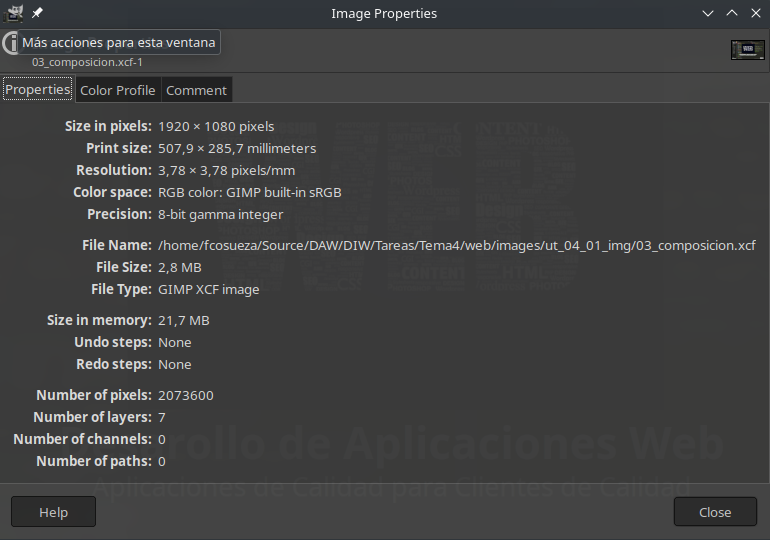
\includegraphics[scale=0.43]{propiedades.png}
\end{figure}

El \textbf{formato} elegido para la composición final ha sido \textbf{WebP}. Se ha elegido este formato porque genera archivos que en relación a su reducido tamaño, tienen más calidad que PNG.

Si bien es cierto que la gran mayoría de navegadores soportan este formato, hay alguno, en concreto Internet Explorer, que no lo soporta aún, como podemos ver en \href{https://caniuse.com/webp}{Can I Use}. Si se tiene mucho interés en dar soporte a este navegador, se podría crear una imagen alternativa y crear una media query para que cargue la imagen en otro formato, pero en general, con este formato tenemos más ventajas que inconvenientes.

\section{Ejercicio 2: Imagen Transformación y Optimización}
En este apartado vamos a realizar alguna transformación en la composición creada y a reducir un poco su tamaño, que ya de pos sí es bastante bajo. Para realizar la reducción de tamaño se ha realizado lo siguiente:

\begin{itemize}
    \item \textbf{Reducción de Tamaño}: la propia reducción de tamaño que se nos ha solicitado en el enunciado ya nos ha servido para reducir su peso considerable, así que esta ha sido la primera medida que se ha tomado.
    \item \textbf{Bajara la Calidad}: la segunda medido ha sido bajar la calidad de la imagen cuando la hemos exportado, tanto de la imagen como del canal Alpha, eso ha supuesto también una reducción del peso de la imagen. Tanto esta media como la anterior se han realizado con GIMP.
\end{itemize}

\section{Ejercicio 3: Audio}
En este ejercicio se ha descargado una canción sin derechos de copyright. En nuestro caso, ha sido la canción \textbf{Sunset Cafe} de \textbf{La Repetición}. Esta canción esta en formato \textbf{MP3} y tiene las licencias \textbf{CC-By} y \textbf{CC-ND}.

Se ha exportado la canción a dos formatos, aunque uno de ellos se ha mantenido como MP3 por el motivo que ahora vamos a explicar. Los formatos a los que se ha exportado son:

\begin{itemize}
    \item \textbf{Ogg Vorbis}: se ha elegido este formato porque con archivos con el mismo tamaño genera mayor calidad que MP3, además de que es un formato bien soportado en los navegadores.

    \item \textbf{MP3}: se ha exportado el archivo a MP3. En original ya estaba en esto formato, pero al exportarlo se ha bajado un poco la calidad, para obtener un archivo que pese un poco menos. Se ha decidido mantener el formato MP3 ya que es el formato de audio digital más soportado por todos los navegadores y dispositivos, por lo que sería oportuno tener un audio en este formato como fallback, para el caso de dar con algún navegador o dispositivo que no soporte Ogg Vorbis.
\end{itemize}

\section{Ejercicio 4: Vídeo}
En este apartado se va a realizar un vídeo explicativo sobre la extensión \textbf{rust-analyzer} de \textbf{VS Code}. Posteriormente, se realizará una composición con este vídeo con el software \textbf{Kdenlive} y se exportará a dos formatos aptos para web.

En primer lugar, se ha posteado en el foro la extensión sobre la que se quiere realizar el vídeo. En un primer momento se pensó en realizarlo sobre \textbf{Emmet}, una extensión para expandir abreviaturas HTML y CSS muy útil para el desarrollo web. El problema, es que en las últimos versión de VS Code esta extensión ha dejado de existir, ya que Emmet viene incorporado por defecto, así que se decidió realizar el vídeo sobre \textbf{rust-analyzer}, una extensión que proporcionar soporte para el lenguaje de programación Rust. En la siguiente captura, podemos ver en mensaje dejado en el foro.

\begin{figure}[H]
    \centering
    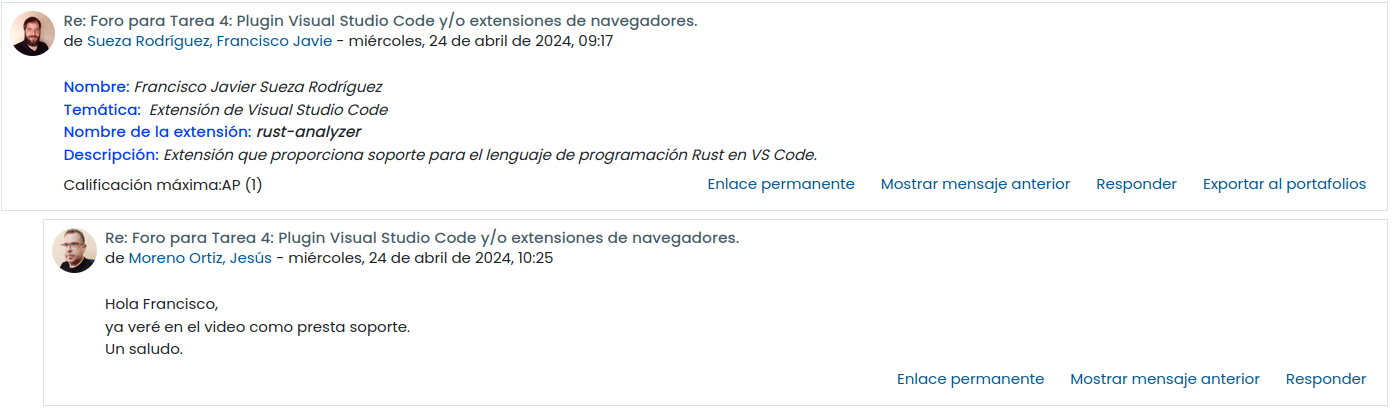
\includegraphics[scale=0.45]{foro.png}
\end{figure}

Se ha decidido, para mantener la uniformidad de licencias del proyecto, emplear la licencia \textbf{CC-Zero}, es decir, de dominio público, como el resto de imágenes y composiciones que se han realizado en esta tarea.

Respecto a la \textbf{transición} utilizada, se ha empleado, en varios puntos del proyecto tanto las transiciones \textbf{fade-in} y \textbf{fade-out}, aunque la que se pedía en concreto entre la imagen de composición y el inicio del vídeo ha sido una transición \textbf{fade-in} con una duración de \textbf{4 segundos}.

El vídeo se ha creado, como ya hemos comentado con \textbf{Kdenlive}, que también ha sido utilizado para su edición. En la siguiente imagen podemos ver la interfaz de Kdenlive con el proyecto finalizado.

Respecto al \textbf{efecto}, se ha utilizado una \textbf{transformación} sobre el \textbf{logo del IES Aguadulce}, reduciendo su tamaño y situándola en la esquita superior izquierda, además de un \textbf{efecto de realce}, incremetando la gamma del logo. Estos efectos se pueden ver todo el tiempo que esta visible el logo, desde sel \textbf{segundo 20} al \textbf{40}.

\begin{figure}[H]
    \centering
    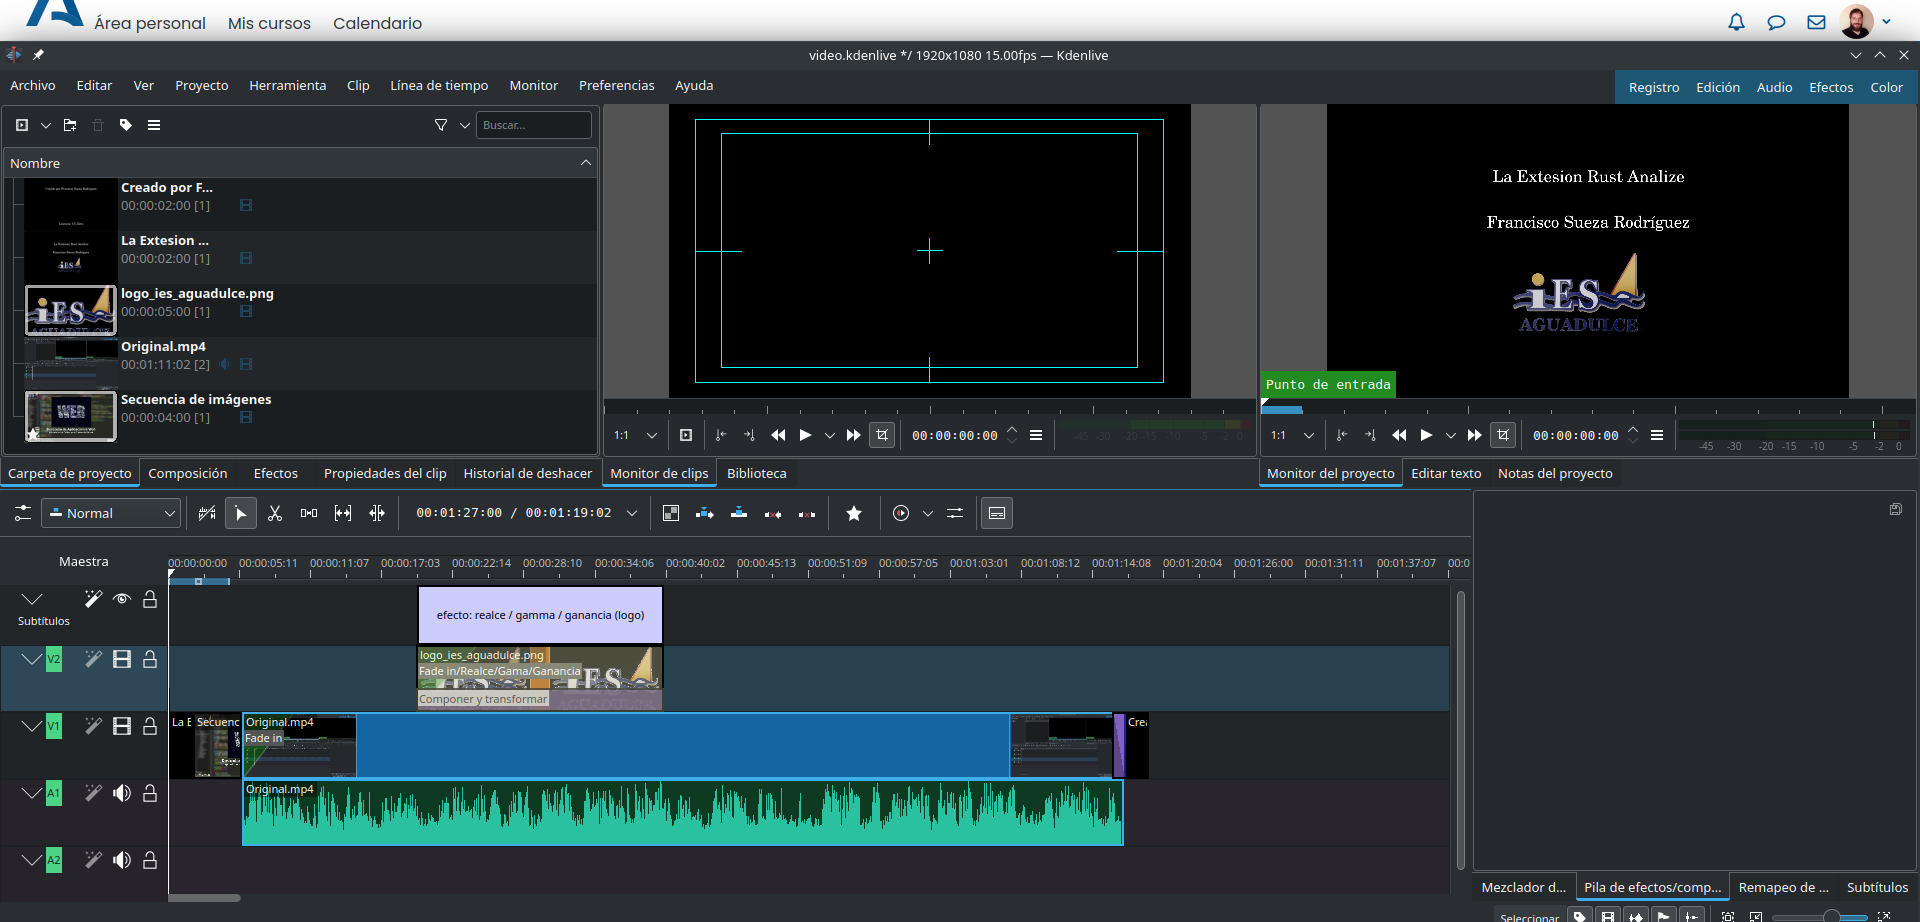
\includegraphics[scale=0.30]{captura-kden.png}
\end{figure}

Ya que en la captura anterior no se aprecia con claridad, se ha realizado una segunda captura mas detallada de la línea de tiempo del proyecto para que se puedan apreciar las diferentes transiciones, que podemos ver como \textbf{triángulos rojos} (fade-out) o \textbf{verdes} (fade-in) al inicio de cada segmento de vídeo. Si nos fijamos, después de la imagen de composición podemos ver el triángulo verde en el inicio del vídeo, así como el nombre del efecto aplicado al logo.

\begin{figure}[H]
    \centering
    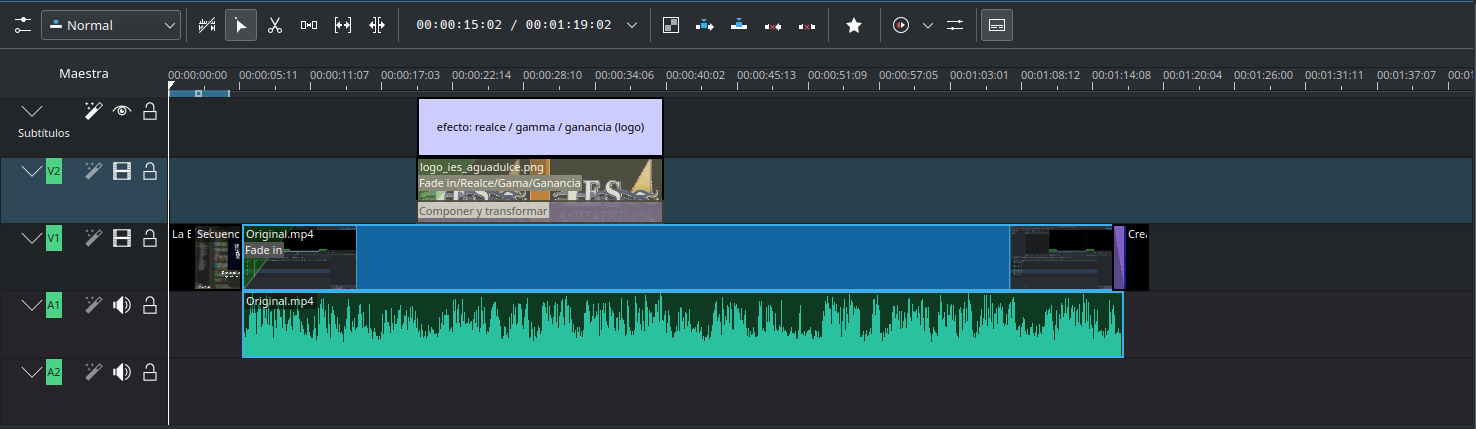
\includegraphics[scale=0.38]{captura-linea.png}
\end{figure}


El vídeo original se ha creado en formato \textbf{MP4}. Una vez editado, se ha exportado el proyecto a dos formatos:

\begin{itemize}
    \item \textbf{MP4}: en uno de los archivos se ha mantenido el mismo formato MP4, por lo ampliamente soportado y utilizado que ésta este formato. Además, tiene buena calidad de imagen.

    \item \textbf{WebM}: es segundo formato ha sido , que produce archivos de gran calidad, con tamaños reducidos usando para ello VP8 para codificación de vídeo y Ogg Vorbis para el audio.
\end{itemize}

\section{Ejercicio 6: Web}
Una vez generados todos los archivos, se ha realizado al web siguiendo las indicaciones. A continuación se muestra una captura de pantalla de la página principal de la web.

\begin{figure}[H]
    \centering
    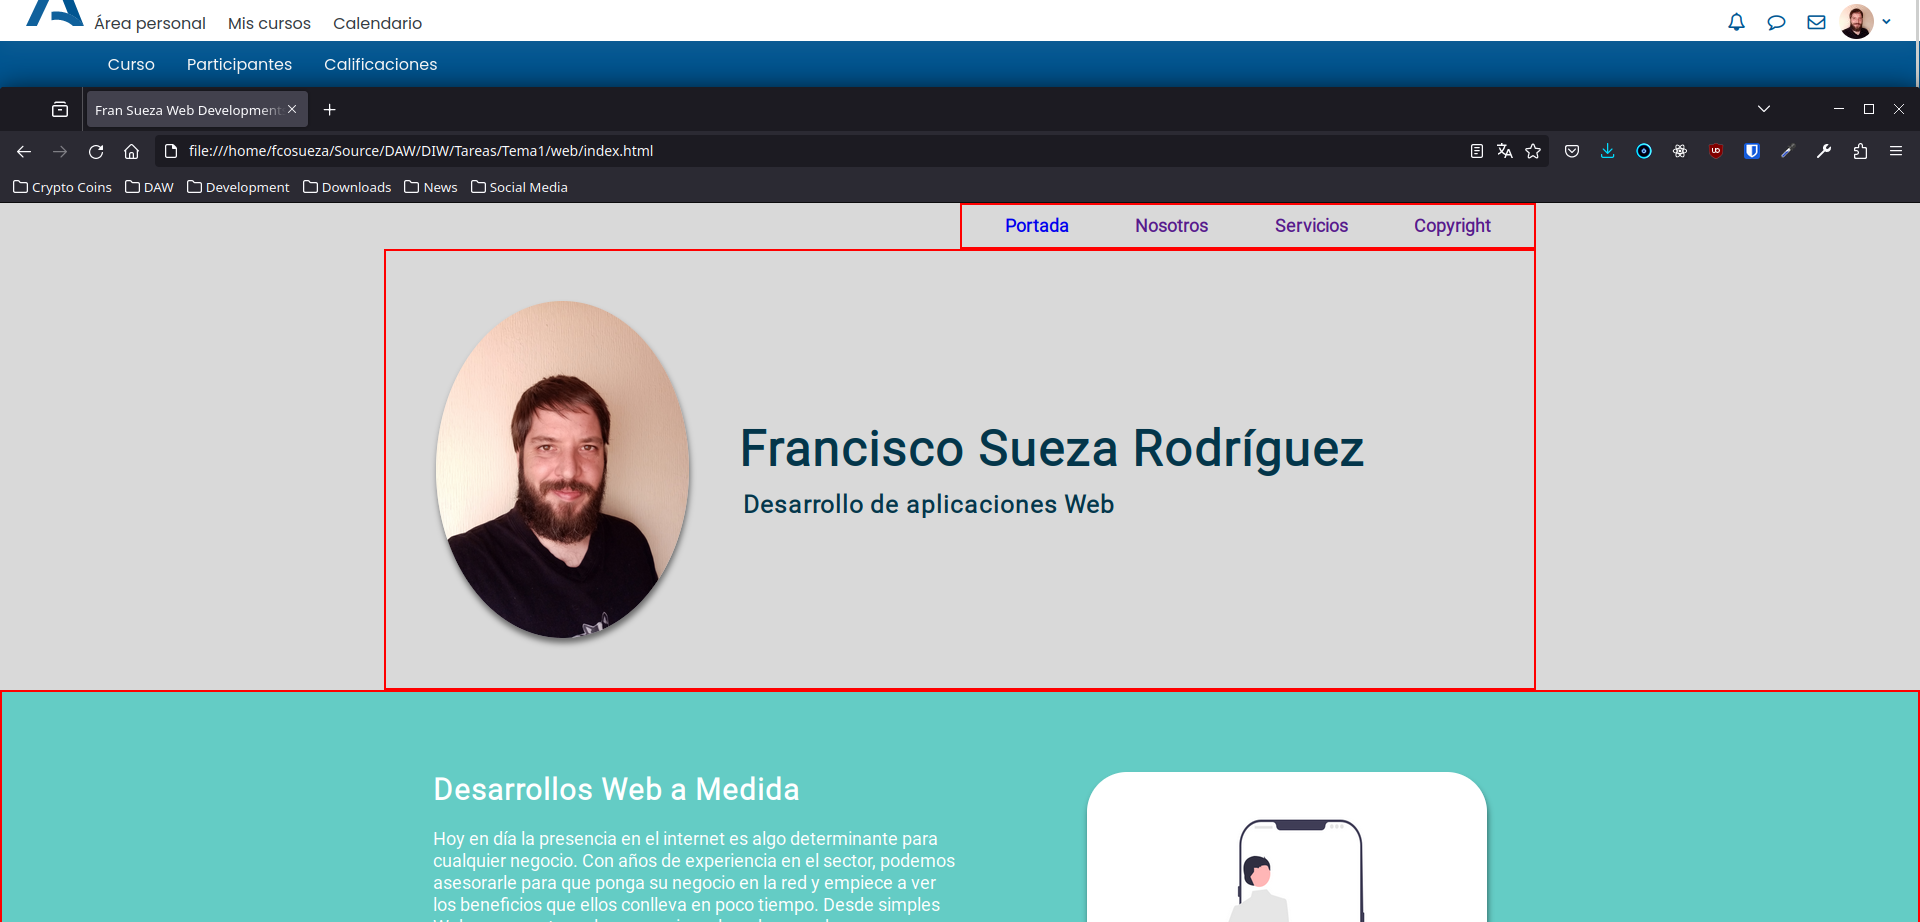
\includegraphics[scale=0.30]{web.png}
\end{figure}

Además, se ha completado la tabla con toda la información de los archivos multimedia generados, que podemos ver a continuación.

\begin{figure}[H]
    \centering
    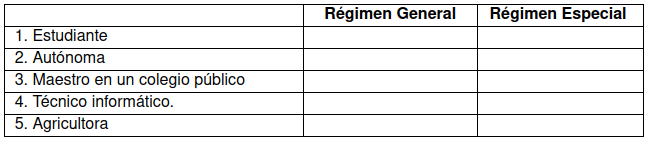
\includegraphics[scale=0.55]{tabla.png}
\end{figure}

% Bibliography

%\newpage
%\bibliography{citas}
%\bibliographystyle{unsrt}

\end{document}